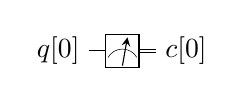
\begin{tikzpicture}[scale=1.000000,x=1pt,y=1pt]
\filldraw[color=white] (0.000000, -7.500000) rectangle (24.000000, 7.500000);
% Drawing wires
% Line 2: q0 W q[0] c[0]
\draw[color=black] (0.000000,0.000000) -- (12.000000,0.000000);
\draw[color=black] (12.000000,-0.500000) -- (24.000000,-0.500000);
\draw[color=black] (12.000000,0.500000) -- (24.000000,0.500000);
\draw[color=black] (0.000000,0.000000) node[left] {$q[0]$};
% Done with wires; drawing gates
% Line 3: q0 M %% as the \\ final op. \\ on q[0]
%\draw (12.000000, -7.500000) node[text width=120pt,below,text centered] {\scriptsize as the \\ final op. \\ on q[0]};
\draw[fill=white] (6.000000, -6.000000) rectangle (18.000000, 6.000000);
\draw[very thin] (12.000000, 0.600000) arc (90:150:6.000000pt);
\draw[very thin] (12.000000, 0.600000) arc (90:30:6.000000pt);
\draw[->,>=stealth] (12.000000, -5.400000) -- +(80:10.392305pt);
% Done with gates; drawing ending labels
\draw[color=black] (24.000000,0.000000) node[right] {$c[0]$};
%\draw (55.000000, 5.00000) node[text width=144pt,below,text centered] {\scriptsize or};
% Done with ending labels; drawing cut lines and comments
% Done with comments
\end{tikzpicture}
